%  template.tex for Biometrics papers
%
%  This file provides a template for Biometrics authors.  Use this
%  template as the starting point for creating your manuscript document.
%  See the file biomsample.tex for an example of a full-blown manuscript.

%  ALWAYS USE THE referee OPTION WITH PAPERS SUBMITTED TO BIOMETRICS!!!
%  You can see what your paper would look like typeset by removing
%  the referee option.  Because the typeset version will be in two
%  columns, however, some of your equations may be too long. DO NOT
%  use the \longequation option discussed in the user guide!!!  This option
%  is reserved ONLY for equations that are impossible to split across 
%  multiple lines; e.g., a very wide matrix.  Instead, type your equations 
%  so that they stay in one column and are split across several lines, 
%  as are almost all equations in the journal.  Use a recent version of the
%  journal as a guide. 
%  
\documentclass[useAMS,referee, usegraphicx]{biom}
%\documentclass[useAMS, usegraphicx]{biom}
%
%  If your system does not have the AMS fonts version 2.0 installed, then
%  remove the useAMS option.
%
%  useAMS allows you to obtain upright Greek characters.
%  e.g. \umu, \upi etc.  See the section on "Upright Greek characters" in
%  this guide for further information.
%
%  If you are using AMS 2.0 fonts, bold math letters/symbols are available
%  at a larger range of sizes for NFSS release 1 and 2 (using \boldmath or
%  preferably \bmath).
% 
%  Other options are described in the user guide. Here are a few:
% 
%  -  If you use Patrick Daly's natbib  to cross-reference your 
%     bibliography entries, use the usenatbib option
%
%  -  If you use \includegraphics (graphicx package) for importing graphics
%     into your figures, use the usegraphicx option
% 
%  If you wish to typeset the paper in Times font (if you do not have the
%  PostScript Type 1 Computer Modern fonts you will need to do this to get
%  smoother fonts in a PDF file) then uncomment the next line
%  \usepackage{Times}
\usepackage{amsmath}
\usepackage{graphicx}
\usepackage{url}

%%%%% PLACE YOUR OWN MACROS HERE %%%%%

\def\bSig\mathbf{\Sigma}
\newcommand{\VS}{V\&S}
\newcommand{\tr}{\mbox{tr}}

%  The rotating package allows you to have tables displayed in landscape
%  mode.  The rotating package is NOT included in this distribution, but
%  can be obtained from the CTAN archive.  USE OF LANDSCAPE TABLES IS
%  STRONGLY DISCOURAGED -- create landscape tables only as a last resort if
%  you see no other way to display the information.  If you do do this,
%  then you need the following command.

%\usepackage[figuresright]{rotating}

%%%%%%%%%%%%%%%%%%%%%%%%%%%%%%%%%%%%%%%%%%%%%%%%%%%%%%%%%%%%%%%%%%%%%

%  Here, place your title and author information.  Note that in 
%  use of the \author command, you create your own footnotes.  Follow
%  the examples below in creating your author and affiliation information.
%  Also consult a recent issue of the journal for examples of formatting.

\title[Mixture model detection functions]{Mixture models for distance sampling detection functions}

%  Here are examples of different configurations of author/affiliation
%  displays.  According to the Biometrics style, in some instances,
%  the convention is to have superscript *, **, etc footnotes to indicate 
%  which of multiple email addresses belong to which author.  In this case,
%  use the \email{ } command to produce the emails in the display.

%  In other cases, such as a single author or two authors from 
%  different institutions, there should be no footnoting.  Here, use
%  the \emailx{ } command instead. 

%  The examples below corrspond to almost every possible configuration
%  of authors and may be used as a guide.  For other configurations, consult
%  a recent issue of the the journal.

%  Single author -- USE \emailx{ } here so that no asterisk footnoting
%  for the email address will be produced.

%\author{John Author\emailx{email@address.edu} \\
%Department of Statistics, University of Warwick, Coventry CV4 7AL, U.K.}

%  Two authors from the same institution, with both emails -- use
%  \email{ } here to produce the asterisk footnoting for each email address

%\author{John Author$^{*}$\email{author@address.edu} and
%Kathy Authoress$^{**}$\email{email2@address.edu} \\
%Department of Statistics, University of Warwick, Coventry CV4 7AL, U.K.}

%  Exactly two authors from different institutions, with both emails  
%  USE \emailx{ } here so that no asterisk footnoting for the email address
%  is produced.

%\author
%{John Author\emailx{author@address.edu} \\
%Department of Statistics, University of Warwick, Coventry CV4 7AL, U.K. 
%\and
%Kathy Author\emailx{anotherauthor@address.edu} \\
%Department of Biostatistics, University of North Carolina at Chapel Hill, 
%Chapel Hill, North Carolina, U.S.A.}

%  Three or more authors from same institution with all emails displayed
%  and footnoted using asterisks -- use \email{ } 

%\author{John Author$^*$\email{author@address.edu}, 
%Jane Author$^{**}$\email{jane@address.edu}, and 
%Dick Author$^{***}$\email{dick@address.edu} \\
%Department of Statistics, University of Warwick, Coventry CV4 7AL, U.K}

%  Three or more authors from same institution with one corresponding email
%  displayed

\author{David L. Miller$^{*}$\email{dave@ninepointeightone.net}, 
Len Thomas\\
Centre for Research into Ecological and Environmental Modelling,\\
University of St Andrews, The Observatory, Buchanan Gardens, St Andrews KY16 9LZ, Scotland}

%  Three or more authors, with at least two different institutions,
%  more than one email displayed 

%\author{John Author$^{1,*}$\email{author@address.edu}, 
%Kathy Author$^{2,**}$\email{anotherauthor@address.edu}, and 
%Wilma Flinstone$^{3,***}$\email{wilma@bedrock.edu} \\
%$^{1}$Department of Statistics, University of Warwick, Coventry CV4 7AL, U.K \\
%$^{2}$Department of Biostatistics, University of North Carolina at 
%Chapel Hill, Chapel Hill, North Carolina, U.S.A. \\
%$^{3}$Department of Geology, University of Bedrock, Bedrock, Kansas, U.S.A.}

%  Three or more authors with at least two different institutions and only
%  one email displayed

%\author{John Author$^{1,*}$\email{author@address.edu}, 
%Wilma Flinstone$^{2}$, and Barney Rubble$^{2}$ \\
%$^{1}$Department of Statistics, University of Warwick, Coventry CV4 7AL, U.K \\
%$^{2}$Department of Geology, University of Bedrock, Bedrock, Kansas, U.S.A.}


\begin{document}

%  This will produce the submission and review information that appears
%  right after the reference section.  Of course, it will be unknown when
%  you submit your paper, so you can either leave this out or put in 
%  sample dates (these will have no effect on the fate of your paper in the
%  review process!)

%\date{{\it Received October} 2007. {\it Revised February} 2008.  {\it Accepted March} 2008.}

%  These options will count the number of pages and provide volume
%  and date information in the upper left hand corner of the top of the 
%  first page as in published papers.  The \pagerange command will only
%  work if you place the command \label{firstpage} near the beginning
%  of the document and \label{lastpage} at the end of the document, as we
%  have done in this template.

%  Again, putting a volume number and date is for your own amusement and
%  has no bearing on what actually happens to your paper!  

%\pagerange{\pageref{firstpage}--\pageref{lastpage}} 
%\volume{65}
%\pubyear{2008}
%\artmonth{December}

%  The \doi command is where the DOI for your paper would be placed should it
%  be published.  Again, if you make one up and stick it here, it means 
%  nothing!

%\doi{10.1111/j.1541-0420.2005.00454.x}

%  This label and the label ``lastpage'' are used by the \pagerange
%  command above to give the page range for the article.  You may have 
%  to process the document twice to get this to match up with what you 
%  expect.  When using the referee option, this will not count the pages
%  with tables and figures.  

\label{firstpage}

%  put the summary for your paper here

\begin{abstract}
This version: \today %Remove this before submitting!

[[Dave: Look at the 3rd panel for Figure 5, (and to a lesser extent the second panel), and the 2nd panel for Figure 6.  The lines do not fit the histograms, nor can any kind of average of them equal the average detection function.  I think the problem is the covariate value of the ``other'' covariate, isn't it?  Can you look into this again and come up with something that looks better?  In mcds.exe we simply don't plot the underlying histogram!  But some kind of average of the plots in Distance would equal the average detection function, so that isn't going to be the whole solution, even if you do decide to do that.  We need somethiing that isn't going to cause a reviewer to say ``that's strange!'']]

We present a new class of models for the detection function in distance sampling surveys of wildlife populations, based on finite mixtures of simple parametric key functions such as the half-normal. The models share many of the features of the widely-used key function plus series expansion formulation: they are flexible, produce plausible shapes with a small number of parameters, allow incorporation of covariates in addition to distance and can be fit using maximum likelihood. One advantage over current methods is the mixtures are automatically monotonic non-increasing and non-negative, so constrained optimization is not required. The mixture formulation is compared to existing methods using extensive simulations and small case studies on real data. [[TKTKTK need to finish by reporting more on our results]]

  
\end{abstract}

%  Please place your key words in alphabetical order, separated
%  by semicolons, with the first letter of the first word capitalized,
%  and a period at the end of the list.
%

\begin{keywords}
Continuous mixture; Finite mixture; Line transect sampling; Monotonicity constraints; Multiple covariate distance sampling; Point transect sampling.
\end{keywords}

%  As usual, the \maketitle command creates the title and author/affiliations
%  display 

\maketitle


%  If you are using the referee option, a new page, numbered page 1, will
%  start after the summary and keywords.  The page numbers thus count the
%  number of pages of your manuscript in the preferred submission style.
%  Remember, ``Normally, regular papers exceeding 25 pages and Reader Reaction 
%  papers exceeding 12 pages in (the preferred style) will be returned to 
%  the authors without review. The page limit includes acknowledgements, 
%  references, and appendices, but not tables and figures. The page count does 
%  not include the title page and abstract. A maximum of six (6) tables or 
%  figures combined is often required.''

%  You may now place the substance of your manuscript here.  Please use
%  the \section, \subsection, etc commands as described in the user guide.
%  Please use \label and \ref commands to cross-reference sections, equations,
%  tables, figures, etc.
%
%  Please DO NOT attempt to reformat the style of equation numbering!
%  For that matter, please do not attempt to redefine anything!

\section{Introduction}
\label{s:intro}


Distance sampling (Buckland et al., 2001, 2004) is a suite of methods for estimating the size or density of biological populations.  There are two main variants, line and point transects. The basic idea is the same in both: an observer visits a randomly-located set of transect lines or points and records the distance, $y$, from the transect to each objects of interest (i.e., animals or plants of the target species) that is detected within some truncation distance $w$.  Not all objects within $w$ are assumed to be detected; instead the observed distances are used to estimate the parameters, $\bm{\theta}$, of a detection function model , $g(y;\bm{\theta})$, which describes how the probability of detection declines with increasing distance.  An assumption of the basic method is that $g(0;\bm{\theta})=1$. Given estimates of $\bm{\theta}$, it is straightforward to estimate population size or density (see Section \ref{s:popsize}).

A key part of distance sampling, therefore, is specification of the detection function model.  Buckland et al. (2001, Chapter 2) provide a set of criteria for judging the utility of candidate model classes: models needs to be flexible, so that they can take a wide variety of shapes, but efficient in the sense of representing plausible shapes with few parameters; they should be flat at zero distance (i.e., $g'(0;\bm{\theta})=0$), and monotonic non-increasing with increasing distance (i.e., $g'(y;\bm{\theta}) \leq 0$ for $0<y\leq w$).  The authors recommend a semiparametric modelling approach developed by Buckland (1992), and this approach has become by far the most popular in practice, partly due to its inclusion in the industry-standard distance sampling analysis software Distance (Thomas et al., 2010).  However, as we demonstrate below, the approach has some drawbacks.  Our purpose in this paper is to propose an alternative class of models, based on mixtures, and to evaluate their utility.

The approach of Buckland (1992) was extended by Marques and Buckland (2004) to allow covariates in addition to distance to be included in the detection function, and, for maximum generality, it is this formulation that we describe here.  The detection function is thus denoted $g(y, \mathbf{z};\bm{\theta})$ where $\mathbf{z}$ is an observation-specific vector of covariates.  The formulation of Buckland (1992) is simply the special case where there are no additional covariates.

In Marques and Buckland (2004), the detection function is modelled as a parametric key function $k$ and series expansion $s$ of even functions (known as adjustment terms) with some parameters $\bm{\theta}$. $g$ is then written as:
\begin{equation*}
g(y, \mathbf{z}; \bm{\theta}) = \frac{k(y, \mathbf{z}; \bm{\theta}) \{1+s(y, \mathbf{z}; \bm{\theta})\}}{k(0, \mathbf{z}; \bm{\theta}) \{1+s(0, \mathbf{z}; \bm{\theta})\}},
\end{equation*}
where $k$ may be a half-normal, hazard-rate or uniform function and $s$ may be zero (i.e., there are no adjustment terms), cosine, simple even polynomial or Hermite polynomial series. The denominator ensures that detection at zero distance is certain (i.e., $g(0, \mathbf{z};\bm{\theta})=1$).  Models are fit to the distance data using maximum likelihood.  The recommended strategy for most situations is to choose a small set of key function and adjustment combinations, and for each combination to choose the number of adjustment terms using forward selection, i.e., start with no adjustment terms and fit an increasing number of terms, stopping when the Akaike Information Criterion (AIC) fails to decrease.  The combination with the lowest AIC is then selected as the best model.  This strategy works well in practice in many cases: the key functions cover a range of realistic shapes for the detection function, so that often zero or one adjustments are sufficient to provide a good fit to the data, resulting in flexible and yet efficient estimation.  The functions are also flat at zero distance, and the key functions are non-increasing.  However, with the addition of adjustment terms, the resulting function is not necessarily non-increasing, nor does it necessarily lie within the interval $[0,1]$.  The solution to this implemented by default in Distance, when there are no additional covariates, is to use constrained maxmimizaion, taking 10 equally spaced distances $y_1=0, \ldots , y_{10}=w$ and ensuring that $g(y_i;\bm{\hat{\theta}})\geq g(y_{i+1}; \bm{\hat{\theta}})$ and that $g(y_{i+1};\bm{\hat{\theta}})\geq 0$ for $i=1,\ldots,9$.

This solution presents a number of problems. Firstly, constrained maximization is a harder problem, meaning in practice that optimization algorithms may fail to find the maximum.  Secondly, constrained maximum likelihood estimates do not have the same appealing properties as their unconstrained cousins -- for example the usual estimator of the standard error of the parameters (square root of the inverse of the information matrix) can be biased.  Thirdly, constraints can only be applied at a finite number of points (10 in the case of Distance), which can lead to the constraint points missing non-monotonic parts of the function.  An example from the recent literature (Williams and Thomas, 2007) is shown in the left panel of Figure \ref{fig1}.  Lastly, it is not clear how to implement the constraints in the case where there are additional covariates, particularly continuous covariates.  One (computationally expensive) option would be to apply the constraints at every observed covariate combintion; however at present Distance uses unconstrained optimization when additional covariates are in the model.  Difficulties arising from this are illustrated in the central and right panels of Figure \ref{fig1} (from Pike et al., 2003), where a strongly non-monotonic function has been fit for some covariate values.  Detection probability estimates outside the range [0,1] are sometimes encountered in Distance during maximization with covariates (in which case the fitting algorithms fail).  Given all of the above, it may be preferable to use a formulation that guarantees monotonicity from the outset.

\begin{figure}
\centering
\includegraphics[width=\textwidth]{figs/figure1.eps}
\caption{Two examples of detection functions that are not monotone, fit using conventional methods in Distance. The first panel is data from humpback whale (Williams and Thomas, 2007): a half-normal detection function with cosine adjustments provided the best fit to the data but, even with constraints in place, the detection function is non-monotonic, with a small secondary peak at approx. 1500m. The second and third panels are data from long-finned pilot whale (Pike et al., 2003) where again a half-normal plus cosine model was fit, but with Beaufort sea state as a covariate and no monotonicity constraints since they cannot be used for multiple covariate models in Distance.  The middle panel shows the detection function averaged over the covariate values and the left panel the marginal detection function for 25th, 50th and 75th quantiles of the Beaufort sea state covariate: non-monotonicity occurs at.}
\label{fig1}
\end{figure}

Mixture models have recently been applied in the capture-recapture literature following the work of Pledger (2000), Dorazio and Royle (2003), Pledger (2005) and Morgan \& Ridout (2008). Their main utility in capture-recapture is in better accounting for between-individual heterogeneity, which can cause severe bias if unmodelled (Link, 2003). In distance sampling this problem does not arise, provided that detection at zero distance is certain, the heterogeneity is not extreme, and a flexible detection function model is used (Buckland, 2004, Section 11.12). Mixture models offer the potential for flexible modelling since the individual parts of the mixture model (the mixture components) can be combined in various ways to yeild a great many possible shapes, and yet all of these will be monotonic non-increasing so long as each component is monotonic non-increasing.  This is the motivation behind the work presented here.

In this paper, we introduce a new class of distance sampling detection function models, based on mixtures of simple parametric key functions.  In the next section, we describe the models.  We then illustrate their use in Section 3 by applying them to simulated data, and then to real data from a number of studies in Section 4. We finish with a discussion of the utility of these new methods.


\section{Finite mixture model detection functions}

\subsection{Formulation}
\label{s:detfcts}

Denoting the detection function as $g$, we consider a sum of $J$ mixture components $g_j$, scaled by some mixture proportions $\phi_j$:
\begin{equation*}
g(y,\mathbf{z}; \bm{\theta}, \bm{\phi}) = \sum_{j=1}^J \phi_j g_j(y,\mathbf{z}; \bm{\theta}_j),
\end{equation*}
where $\sum_{j=1}^J \phi_j = 1$. The (radial or perpendicular) distance is denoted $y$, the $\bm{\theta}_j$s are vectors of parameters for function $g_j$, $\bm{\theta}$ is a vector containing of all of the $\bm{\theta}_j$s, $\bm{\phi}$ is a vector of all of the $\phi_j$s, and $\mathbf{z}$ is an a $K$-vector of the associated covariates.  

Here we let the $g_j$s be half-normal functions (although other monotonic functions such as hazard-rate could be chosen and the $g_j$s need not all have the same form), so
\begin{equation*}
g(y,\mathbf{z}; \bm{\theta}, \bm{\phi}) = \sum_{j=1}^J \phi_j \exp \Big( - \frac{y^2}{2\sigma_j^2} \Big).
\end{equation*}
Covariates can be included in a similar way to Marques and Buckland (2004) (see also Marques et al., 2007), where the covariates affect the scale parameter $\sigma$. We assume that each mixture component has a different scale but that the covariates affect the scale parameters in the same way. Other more complex models may be possible.

Following the notation in Marques and Buckland (2004) and using $i$ to subscript each observation, our formulation for the scale parameter $\sigma_{ij}$, is therefore:
\begin{equation*}
\sigma_{ij} = \exp( \beta_{0j} + \sum_{k=1}^K \beta_k z_{ik}),
\end{equation*}
where $z_{ik}$ is the $k^\text{th}$ covariate for the $i^\text{th}$ observation. As an example, for a 2-point mixture with one covariate, the scale parameters take the form
\begin{equation*}
\sigma_{ij} = \exp( \beta_{0j} + \beta_1 z_{i1}),
\end{equation*}
and then $\bm{\theta}_j = (\beta_{0j}, \beta_1)$. 


\subsection{Likelihood}
\label{s:likelihood}

Maximum likelihood estimation is used to estimate the parameters of the detection function. Before we can perform the optimization, we must first formulate a likelihood. Following from Buckland et al (2001, 2004), we can write the pdf of the observed distances ($f(y,\bm{z}; \bm{\theta}) $) as the ratio of the detection function and its integral:
\begin{equation}
f(y,\bm{z}; \bm{\theta}) = \frac{g(y,\bm{z}; \bm{\theta})}{\int_0^w g(y,\bm{z}; \bm{\theta}) \text{d}y}.
\end{equation}
The likelihood can then be formed by taking product of these pdfs over the $n$ observations, as usual.

For line transects, given a set of perpendicular distances $\{x_i; i=1,\ldots,n\}$ and associated covariate vectors $\bm{z}_i$ (which are the rows of the $n \times K$ matrix $\mathbf{Z}$), the likelihood is given by:
\begin{align*}
\mathcal{L}(\bm{\theta},\bm{\phi}; \mathbf{x},\mathbf{Z}) &= \prod_{i=1}^n f(x_i,\bm{z}_i; \bm{\theta},\bm{\phi})\\
&= \prod_{i=1}^n \frac{g(x_i,\bm{z}_i; \bm{\theta},\bm{\phi})}{\mu_i}\\
&= \prod_{i=1}^n \frac{\sum_{j=1}^J \phi_j g_j(x_i,\bm{z}_i; \bm{\theta}_j)}{\mu_i}
\end{align*}
where $\mu_i$, the effective strip width, is given by:
\begin{equation*}
\mu_{i} = \sum_{j=1}^J \phi_j \int_0^w  g_j(x,\bm{z}_i; \bm{\theta}_j) \text{d}x.
\end{equation*}

For point transects, with radial distances $\{r_i; i=1,\ldots,n\}$ and associated covariate vectors $\bm{z}_i$ (which again form the rows of the $n\times K$ matrix $\mathbf{Z}$), the likelihood is:
\begin{align*}
\mathcal{L}(\bm{\theta},\bm{\phi}; \mathbf{r},\mathbf{Z}) &= \prod_{i=1}^n f(r_i,\bm{z}_i; \bm{\theta},\bm{\phi})\\
&= \prod_{i=1}^n \frac{2 \pi r_i g(r_i,\bm{z}_i; \bm{\theta},\bm{\phi})}{\nu_i}\\
&= \prod_{i=1}^n \frac{2 \pi r_i \sum_{j=1}^J \phi_j g_j(r_i,\bm{z}_i; \bm{\theta}_j)}{\nu_i}
\end{align*}
where the effective area of detection, $\nu_i$ is defined as:
\begin{equation*}
\nu_i = 2\pi \sum_{j=1}^J \phi_j \int_0^w  r g_j(r,\bm{z}_i; \bm{\theta}_j) \text{d}r.
\end{equation*}
Parameters are estimated using maximum likelihood. Practicalities associated with this maximization, along with analytic derivatives of the likelihood are described in Web Appendices A and B.

In this paper, we have assumed that the distance data are in the form of ``exact'' distances from detected objects to the transect; an alternative is that distances are grouped into intervals, with pre-defined cutpoints (e.g., 0-10m, 10-20m, etc.), so that the data are the distance interval of each observation.  In this case, a multinomial likelihood is obtained (see, e.g., Buckland et al., 2001, Section 3.3.2).

\subsection{Estimating population size}
\label{s:popsize}

[[Need to edit stuff here now I've edited the intro.]]

As mentioned above, population size can be found using the Horvitz-Thompson-like estimator given in (\ref{HT}). In the mixture model case $p_i$  (the probability of the $i\text{th}$ observation being detected given it is within the sampled area) is given by:
\begin{equation*}
p_i = \frac{1}{w} \sum_{j=1}^J \phi_j \int_0^w  g_j(x,\mathbf{Z}; \bm{\theta}_j) \text{d}x,
\end{equation*}
for line transects and for point transects by
\begin{equation*}
p_i = \frac{2\pi}{w^2} \sum_{j=1}^J \phi_j \int_0^w  r g_j(r,\mathbf{Z}; \bm{\theta}_j) \text{d}r.
\end{equation*}
A standard summary statistic is the average detection probability for an animal within the covered region [[[did you define covered region earlier?]], $P_a$, which is given by:
\begin{equation*}
P_a = n/N.
\end{equation*}
Estimators for the variances of $N$ and $P_a$ are given in Web Appendix E.


\section{Simulations}
\label{s:sims}

Extensive simulations were carried out to investigate performance, in terms of the accuracy of estimation of $P_a$ and $N$, under the circumstance when the true model is not known to the estimation procedure. Each simulation involved generating 200 replicate datasets from a specified mixture model, fitting each dataset with 1-, 2-, and 3-point mixture models for the detection function, and in each case recording estimated parameter values and abundance from the model with the lowest AIC.

[[ Need to add in some blurb about the hazard rate mixtures ]]

Four sets of simulations were run:
\begin{enumerate}
	\item Non-covariate 2-point detection functions for line transect data. Four different detection functions were tested; these are illustrated in the first row of Figure \ref{sim-detfcts}. The first two should be relatively easy to fit. The third should be harder, testing the behaviour of the model when the scale parameter of one of the mixture components is very large relative to the truncation distance. Finally, the fourth detection function has a large spike (i.e., a sharp decline in detectability at small distances), which is similar to that in some of the data we analyse in Section \ref{s:data}.
	\item Non-covariate 2-point detection functions for point transect data.  The detection functions were as above, with data generated as if it came from point transects. The pdfs are given in the second row of Figure \ref{sim-detfcts}.
	\item Non-covariate 3-point detection functions for line transect data. Two different models for the detection functions were used. They are shown in the third row of Figure \ref{sim-detfcts}. The first is much like the second line transect detection function, enabling us to investigate the efficacy of model selection. The second is a more complex shape that could only be created using a 3-point mixture; it has the added complication (as with the third line transect simulation) that one of the components has a large scale parameter relative to truncation distance.
	\item Covariate 2-point detection functions for line transect data. Two different models were tested, the first of which has a binary factor covariate: half of the observations had covariate value 1 and half had covariate value 0. The second model had a continuous covariate, whose values were generated from a standard normal distribution function. Detection functions are shown in the fourth row of Figure \ref{sim-detfcts}, along with the marginal detection functions for the levels/quantiles of the covariates. One goal was to test the properties of the estimator in the presence of covariates, and for these runs we included the covariate in all models fit.  However, we additionally wished to evaluate the performance of the mixture model formulation in cases where a covariate affects detectability but the covariate is not available to the observer.  We therefore fit the same simulated datasets with mixture models that did not include covariates, and compared the resulting estimates to their with-covariate counterparts.
\end{enumerate}

True parameters and average detectabilities are given in Web Appendix C.

\begin{figure}
\centering
\includegraphics[width=\textwidth]{figs/sim-detfct.eps}
\caption{Plots of the models used in the simulation. Top row: detection functions for the line transect simulations with no covariates (solid lines) and their constituent mixture components (dashed lines). Second row: pdfs for the point transect simulations with no covariates (bold lines), with associates component pdfs, rescaled so the area under each curve is one; the detection functions are as in the top row. Third row: two 3-point mixtures for non-covariate line transect data, again with components as dashed lines. Fourth row, two covariate models, the first two panels are for a binary covariate, the second two for a continuous covariate; first panels in each pair show the detection function averaged over the covariates (along with the mixture components, similarly averaged) and the second panels show marginal detection functions with the levels (or quantiles) of the detection function.}
\label{sim-detfcts}
\end{figure}


[[probably need to re-write and/or cut this down]]

Results from the simulation study are shown in Figure \ref{sim-boxplots}. Boxplots are of the estimated average detection probability, $\hat{P_a}$. The number under each boxplot gives the proportion of AIC best models that were of the same form as the true model (i.e. same number of mixture components and same covariates selected). For the first row (line transects with no covariates) we can see that in scenarios 1 and 3, both the true model and true probability of detection were found, even at low sample sizes; whereas in scenarios 2 and 4 there was a positive bias in the estimates of the probability of detection as well as a lower proportion of ``correct'' models being selected by AIC. In scenario 2 and 4 most of the weight (0.7 and 0.6, respectively) is given to the larger mixture component, thus the smaller component is swamped; making the simulated data look as if it were generated from a 1-point mixture.

This effect can also be seen in the point transect simulations, but more severely. In this case one can see from the second row of Figure \ref{sim-detfcts} that the pdfs of the distances look very much like only one of the components of the mixture. Fitting only a 1-point mixture to data from a 2-point mixture has lead to a positive bias in the detection probabilities, however this is only to expected given that data generated from such models would look like a 1-point mixture.

The results from the first of the 3-point mixtures show that detection function can be easily represented using a smaller number of mixture terms. At sample sizes of 120 and lower, a 1-point mixture model dominated (around 150 of the AIC selected models were 1-point mixtures) then at the two higher sample sizes, 2-point mixtures dominated. Scenario 2 is more like a ``true'' 3-point data set, although only at the two larger sample sizes was a 3-point model selected more than half of the time. Note that at the lower sample sizes, a 2-point mixture was selected more often than 1-point (137, 173 and 182 times for the lowest three sample sizes). This effect may be due to the large, potentially non-identifiable, scale parameter being confounded with the other parameters, although this did not appear to be problematic in the scenario 2 of the line transect non-covariate models, above.

The covariate models again show an initial positive bias in the $P_a$ estimates but do still converge to the true value at higher sample sizes (bottom row of Figure \ref{sim-boxplots}). The numbers beneath the boxplots mask rather more for the covariate models than in the other cases, since model selection was performed on not only the number of mixtures but also on the inclusion of covariates. At the larger two sample sizes we see that the ``true'' model is selected almost all of the time. However,  at smaller sample sizes we see more interesting behaviour. For scenario 1, at the two lowest sample sizes a 1-point non-covariate model dominates, followed by 1-point with covariates, then 2-point covariate and 2-point non-covariate. So, as one would expect, the simplest two models are selected most, but the added information from the covariates means that the 2-point covariate is selected ahead of the 2-point non-covariate. At sample size 120, the 1- and 2-point covariate models are both selected about 70 times, and the non-covariate 1- and 2-point models about 30 times. Contrary to expectations the 3-point mixtures are barely selected at all (with or without covariates) leading us to believe that the covariates cannot simply be substituted by further mixture terms, even in the binary covariate case. Scenario 2 shows a slightly different picture; the non-covariate models are selected less, even at lower sample sizes (the 1-point covariate model was selected 90 times a the lowest sample size) which might be expected given that scenario 2 included a continuous covariate. As was the case for scenario 1, the 3-point models were barely selected at all. In both scenarios there seems to be a ``bite point'' between a sample size of 120 and 480 where the correct model is selected almost every time.

[[ For the covariate models, when fitting an MCDS model with covariates, AIC would select non-monotonic models with vastly lower AICs (-2500, next lowest model was -600) with very different abundance estimates. Since we would not select such non-monotone models in a real analysis, the MCDS models were fitted without adjustments. (Maybe say something about Jeff's complaints here, maybe not).]]


Further details of simulation results are given in Web Appendix D.

\begin{figure}
\centering
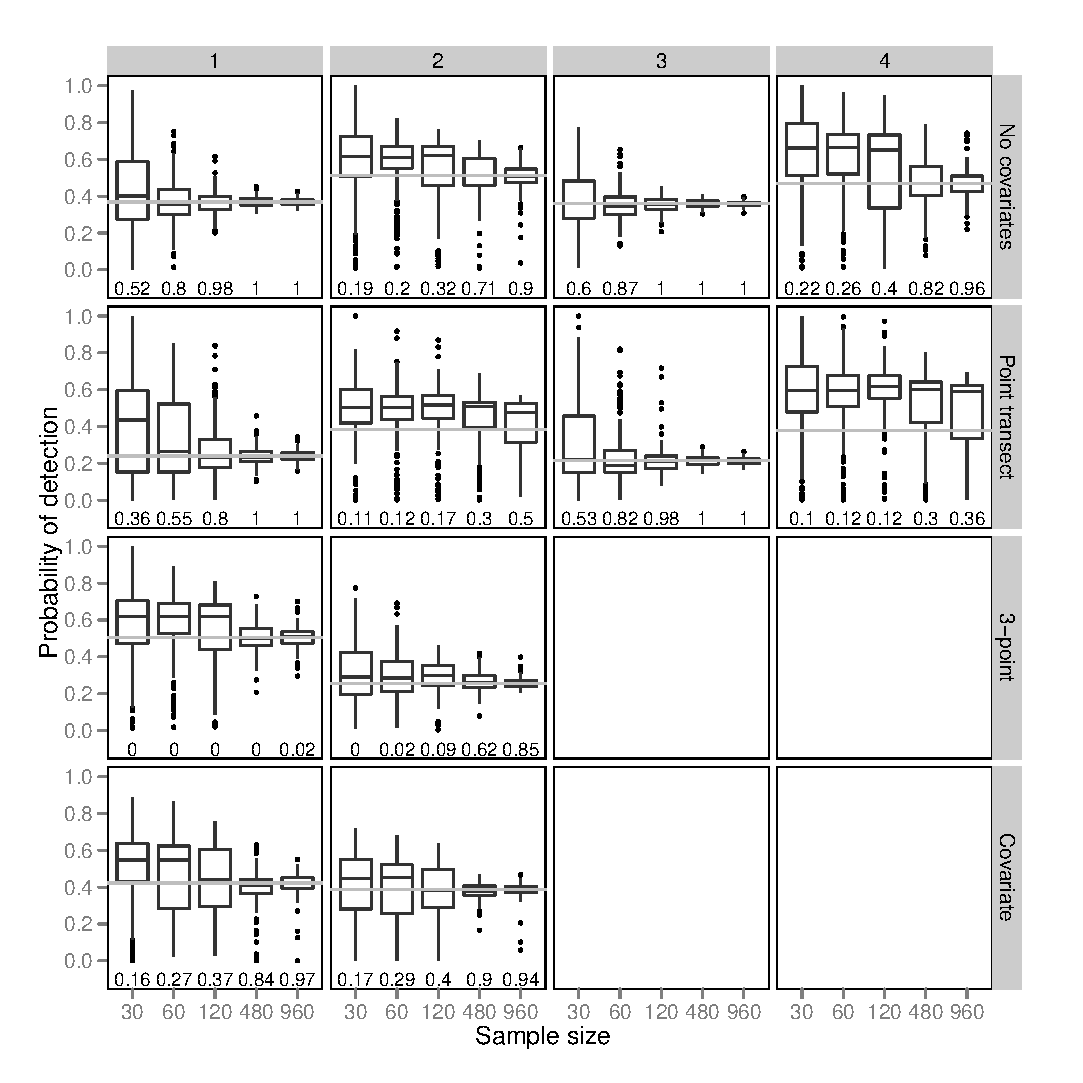
\includegraphics[width=\textwidth]{simulations/pa-plot.eps}
\caption{Simulation results: boxplots of the estimated average detection probabilities, $P_a$, for the best model (by AIC score). Layout is as in Figure \ref{sim-detfcts}. Grey lines indicate the true value of the average detection probability. Numbers underneath each boxplot give the proportion of AIC best models that were of the same form as the model that the data was simulated from (e.g., in covariate case 1 the proportion of AIC best models that were two point mixtures that included the covariate in the model).}
\label{sim-boxplots}
\end{figure}


\section{Case studies}
\label{s:data}

Given the performance of the method in simulation, several data sets were analysed using the method. Analyses were performed in \texttt{mmds} (Mixture Model Distance Sampling), an \textsf{R} package written by the authors and available on CRAN. Results from using mixture model detection functions are compared with those from the original articles.

[[\textbf{LEN}: is further detail needed for any of these?]]

\subsection{Williams and Thomas (2007) cetacean survey}

Williams and Thomas (2007) study several species of cetaceans off the coast of British Columbia. In particular we look at three species: harbour seal (in water), harbour porpoise and humpback whale (with truncation at 500m, 500m and 2000m respectively). Results are summarised in Table \ref{williams-table} and detection functions for the best (in an AIC sense) models are shown in Figure \ref{williams-detfcts}.

\begin{table}
\caption{Comparison of the results for the Williams and Thomas (2007) data. W\&T indicates the results reported in Williams and Thomas (2007), other results are from mixture models where the number of mixture components was selected by AIC. $\cos(x)$ indicates a Cosine adjustment of order $x$.}
\centering
\begin{tabular}{c c c c c c}
\hline \hline
Species & Model & AIC & $\hat{P_a}$ & $\% CV \hat{P_a}$ & K-S $p$\\
\hline
Harbour seal & Hn+$\cos(2)$ (W\&T) & 2771.05 & 0.425 & 7.55 & 0.515\\
(in water) & Hn 2-pt  & 2769.86 & 0.335 & 15.38 & 0.945\\
Harbour porpoise & Hr (W\&T) & 690.66 & 0.212 & 32.0 & 0.99\\
 & Hn 2-pt & 692.09 & 0.254 & 18.18 & 0.99\\
Humpback & Hn+$\cos(2)$ (W\&T) & 1033.06 & 0.386 & 12.64 & 0.672 \\
 & Hn 2-pt & 1035.94 & 0.381 & 18.48 & 0.649 \\
\hline
\end{tabular}
\label{williams-table}
\end{table}

In each case a 2-point mixture was selected by AIC to be the best model. The mixture models for the harbour porpoise and the humpback both did not perform as well as the models selected in Williams and Thomas (2007). However, for the harbour porpoise the AIC is only different by 2, the detectability is very similar and the \%CV is lower, so it does not appear that much is lost by using the mixture model. In the case of the humpback, the fitted detection function is monotone, which was not the case in Williams and Thomas (2007); this added to the fact that there is again not a huge difference in results, leads us to believe that mixture models for the detection function can be useful. Finally, for the harbour seal data, the mixture model had a better AIC than the half-normal with cosine adjustments of order 2 which was selected in the paper. The goodness-of-fit was also significantly better than the result given in Williams and Thomas (2007).

\begin{figure}
\centering
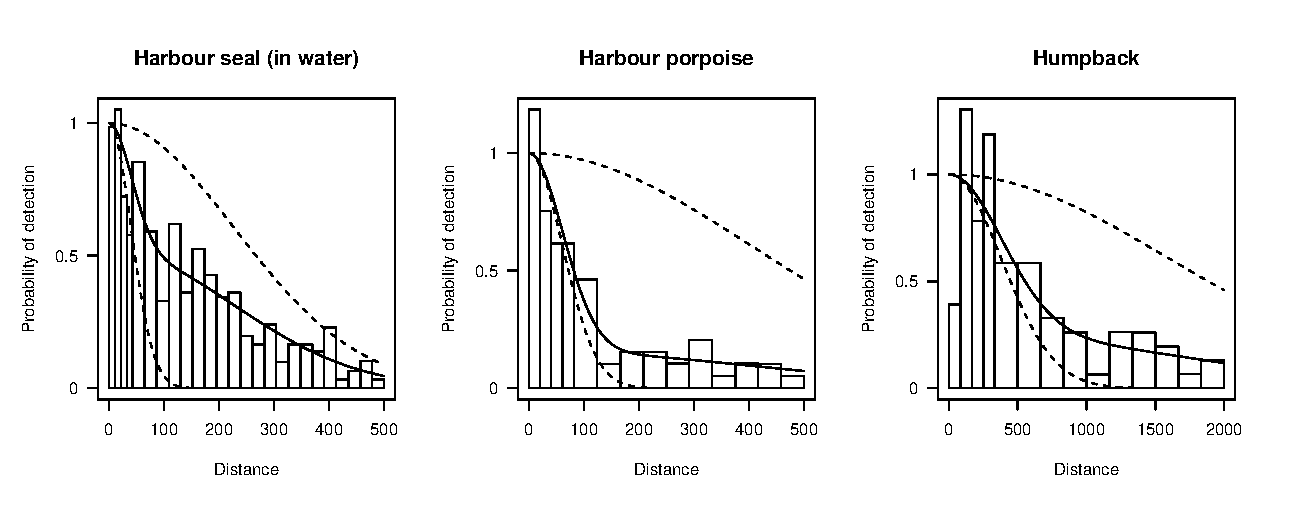
\includegraphics[width=\textwidth]{analyses/williamsplots.eps}
\caption{Plots of the detection functions fit to the Williams and Thomas (2007) data. In each case the best model by AIC was a 2-point mixture. Dashed lines show the mixture components.}
\label{williams-detfcts}
\end{figure}


\subsection{Wood ants in the Abernethy forest}

Borkin, Summers and Thomas (2012) analyse data on two species of wood ant (\textit{Formica aquilonia} and \textit{Formica lugubris}) in the Abernethy Forest in Strathspey Scotland over the period of August--September 2003. The number of nests sighted was 150 out to a distance of 72.04m from the track line, although 45\% of the nest sightings lay within 4m of the line. As part of their analysis several different truncation distances were used and larger truncation distances led to large variance in the encounter rate estimates and hence in overall abundance estimates (see Borkin et al., 2012). This is due to the spike caused by the large number of detections close to the line.

As well as distances, three covariates were recorded: habitat type (\texttt{habitat}, a four level factor), the size (calculated as half-width multiplied by height) of each nest (\texttt{nest.size}, continuous variable) and whether \textit{Formica aquilonia} or \textit{Formica lugubris} were observed (\texttt{species}, a two level factor). In order to avoid numerical problems due to large values of the nest size, the variable was standardised.

As can be seen from Table \ref{big-results-table}, the best model by AIC was a 2-point mixture with nest size and habitat as covariates. This is not that surprising given the best CDS model (selected by AIC) in Distance was a hazard-rate with the same covariates. What is rather surprising is that the best mixture model had a better AIC than the hazard-rate, even though it has 1 more parameter. This is particularly encouraging since one might expect that mixtures would give good fits but would not achieve lower AIC scores due to the number of parameters required.

\begin{figure}
\centering
%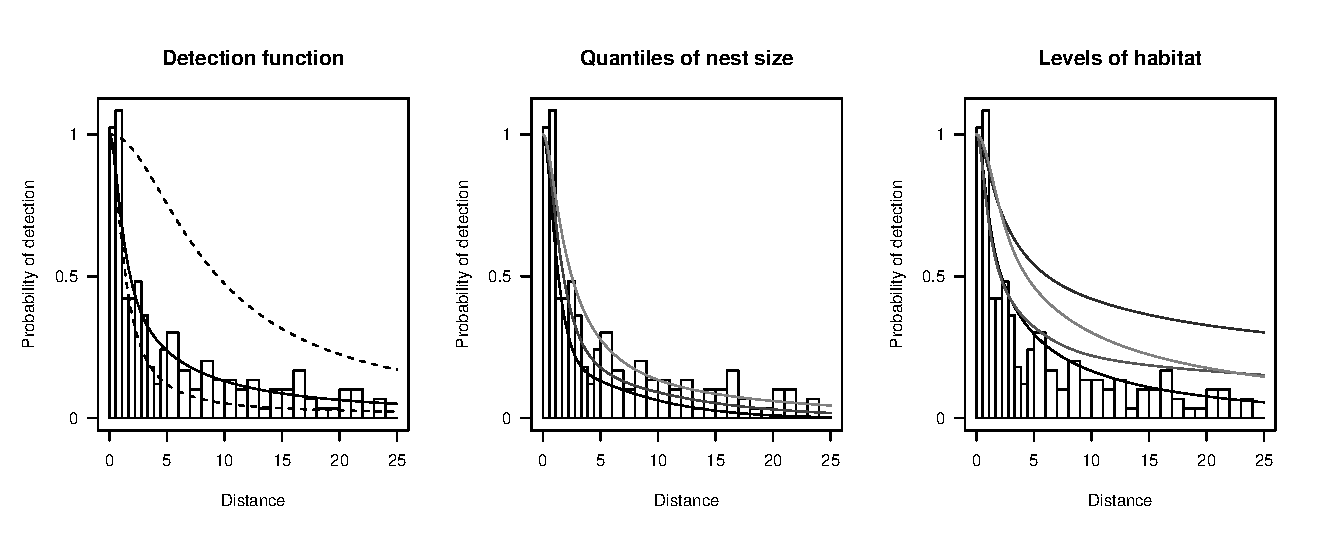
\includegraphics[width=\textwidth]{analyses/ants-nesthab.eps}
\includegraphics[width=0.3333\textwidth, trim=0 0 5.73228347in 0, clip=true]{analyses/ants-nesthab-1.eps}\includegraphics[width=0.6666\textwidth, trim=2.86614173in 0 0 0, clip=true]{analyses/ants-nesthab-2.eps}
\caption{Plot of the detection functions for the AIC best model for the ants data set (2-point mixture with nest size and habitat as covariates). The first panel shows the average detection function (dashed lines are the two mixture components of the detection function, averaged over covariate values). The second and third panels show the quantiles (25\%, 50\% and 75\%) of nest size and the levels of habitat type respectively.}
\label{ants-nesthab}
\end{figure}


\subsection{Long-finned pilot whales}

Pike et al. (2003) analyse data on long-finned pilot whales (\textit{Globicephala melas}). There were 84 pods sighted as part of the NASS-2001 survey (of which the pilot whale was not a target). The Beaufort sea state was recorded as a covariate during the survey and enter the model as either a continuous variable (\texttt{BSS}), 6 level factor (\texttt{BSS}, as a factor), a 2 level factor (\texttt{BSS3}) or a 3 level factor (\texttt{BSS2}).

A model was fit with each of these covariates, as well as a model with no covariates. A summary of the results is given in Table \ref{big-results-table} and the detection function for the best model is shown in Figure \ref{danpike-detfct}.

\begin{figure}
\centering
%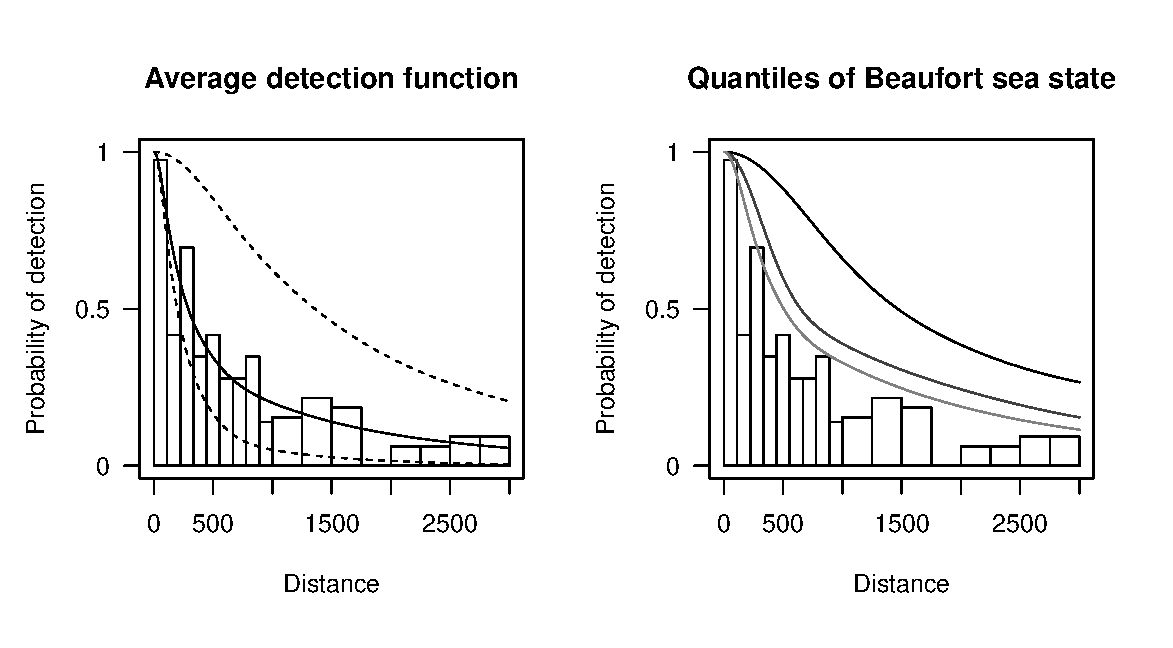
\includegraphics[width=0.75\textwidth]{analyses/danpike-bssc.eps}
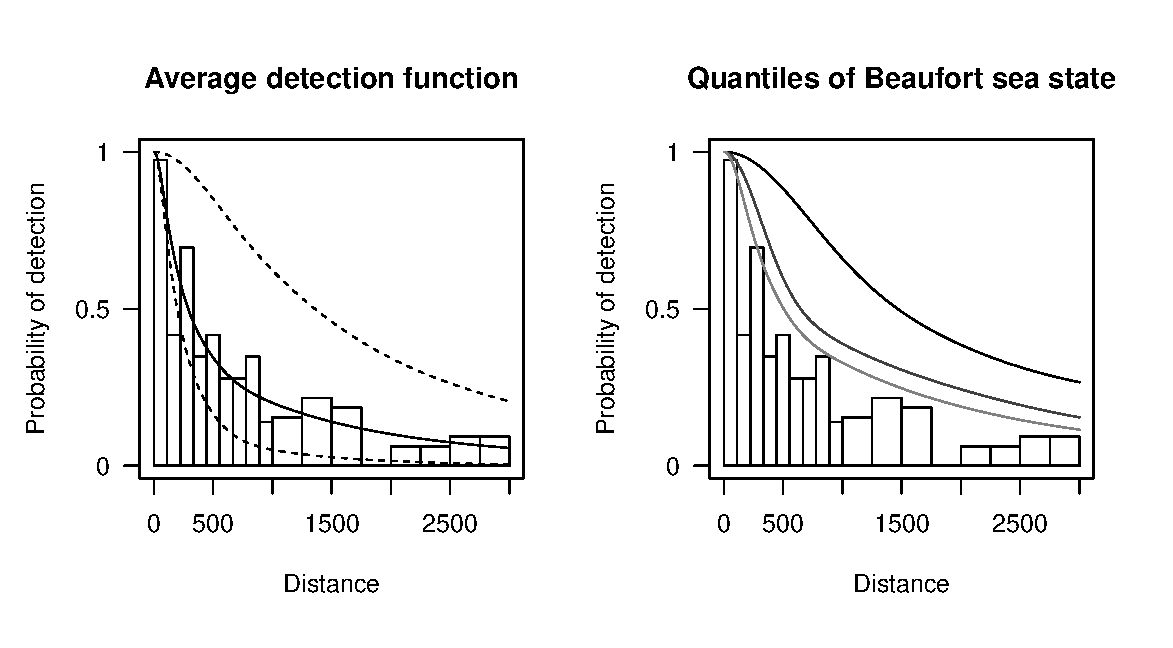
\includegraphics[width=0.375\textwidth, trim= 0 0 3.8in 0, clip=true]{analyses/danpike-bssc.eps}\includegraphics[width=0.375\textwidth, trim= 3.8in 0 0 0, clip=true]{analyses/danpike-bssc-hh.eps}
\caption{The (AIC) best model for the long-finned pilot whale data: a 2-point mixture model detection function with Beaufort sea state as a continuous covariate. Left: the average detection function, right: the marginal detection function with the quantiles (25\%, 50\% and 75\%) of \texttt{BSS}.}
\label{danpike-detfct}
\end{figure}

The best model by AIC score was a 2-point mixture with \texttt{BSS} as a continuous covariate. Figure \ref{danpike-detfct} shows the average detection function and the marginal detection function with the quantiles of \texttt{BSS}. As one would expect, none of the non-monotonic behaviour seen in Figure \ref{fig1} can be seen here.

\subsection{Amakihi}
Marques et al. (2007) analyse data on the Hawaii Amakihi (\textit{Hemignathus virens}). The data consist of 1485 observations on the bird ($n=1243$ after truncation at 82.5m), collected at 41 point transect from July 1992 to April 1995. Data was also collected on three covariates: the observer (\texttt{obs} , a three level factor), minutes after sunrise (\texttt{mas}, continuous, standardised to prevent numerical issues) and hours after sunrise (\texttt{has}, a six level factor).

\begin{figure}
\centering
%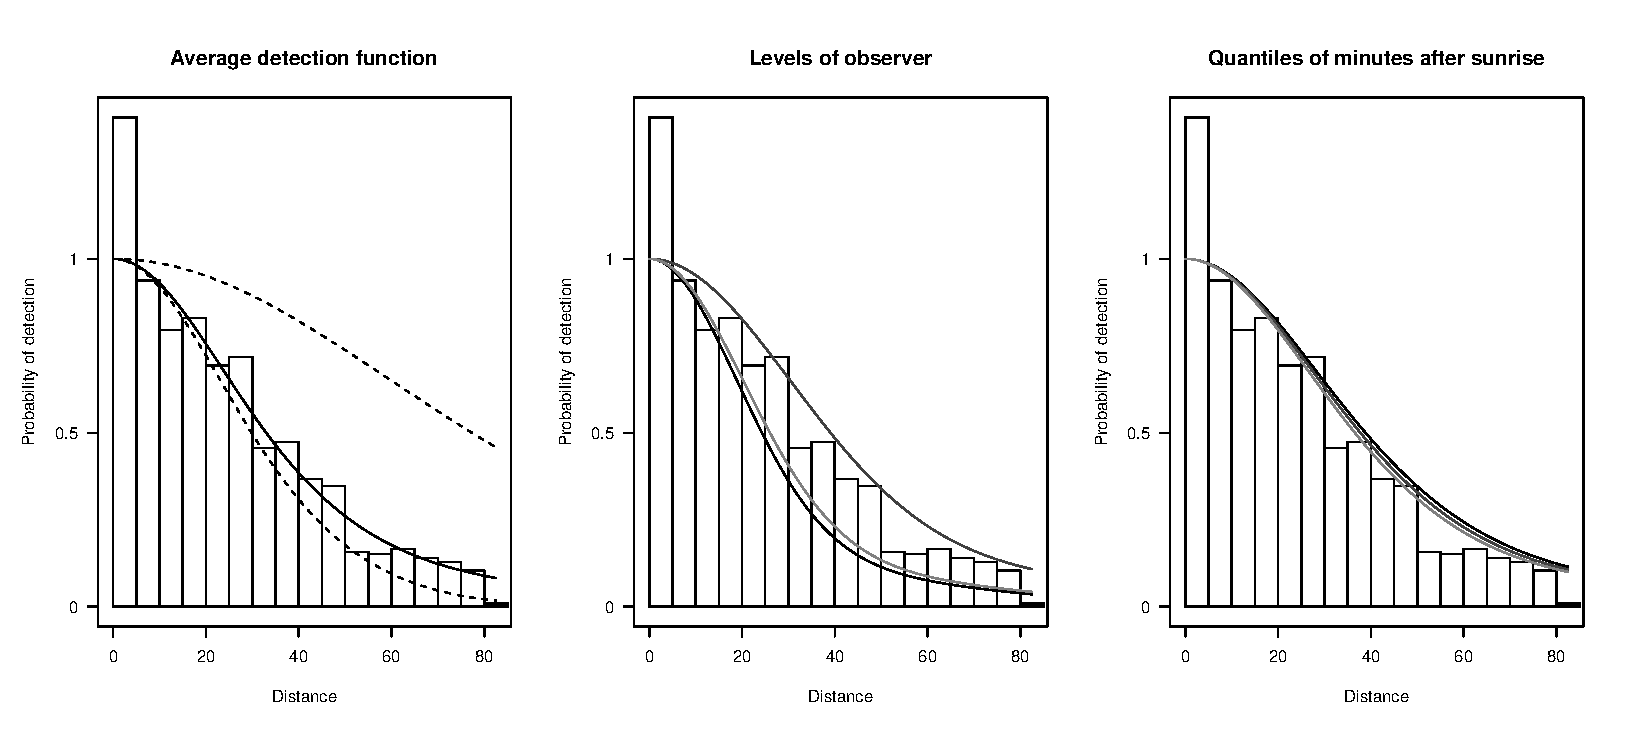
\includegraphics[width=\textwidth]{analyses/amakihi-om.eps}\\
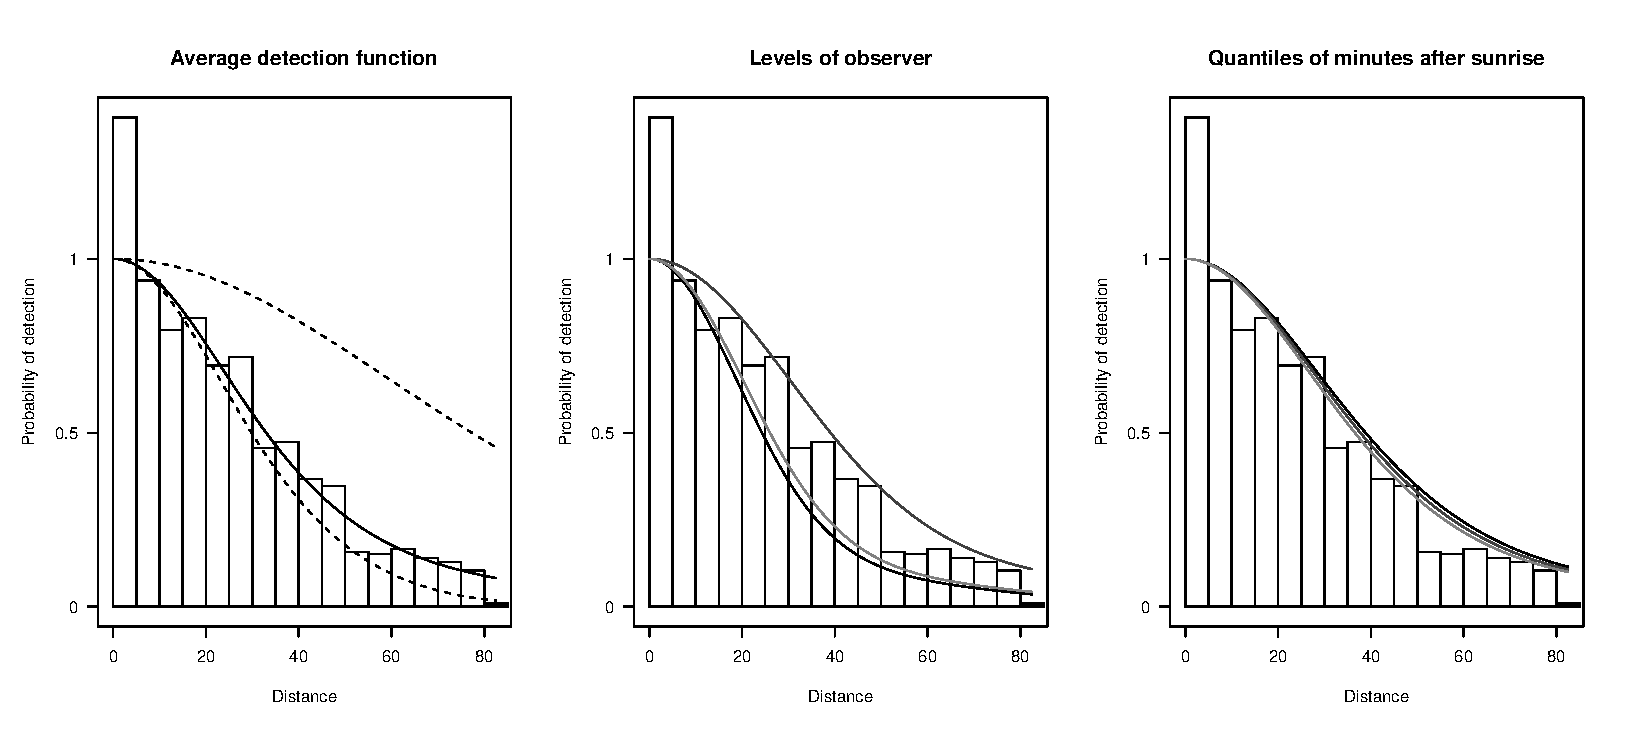
\includegraphics[width=0.3333\textwidth, trim=0 0 7.133334in 0, clip=true]{analyses/amakihi-om.eps}\includegraphics[width=0.6666\textwidth, trim=3.566667in 0 0 0, clip=true]{analyses/amakihi-om-hh.eps}\\
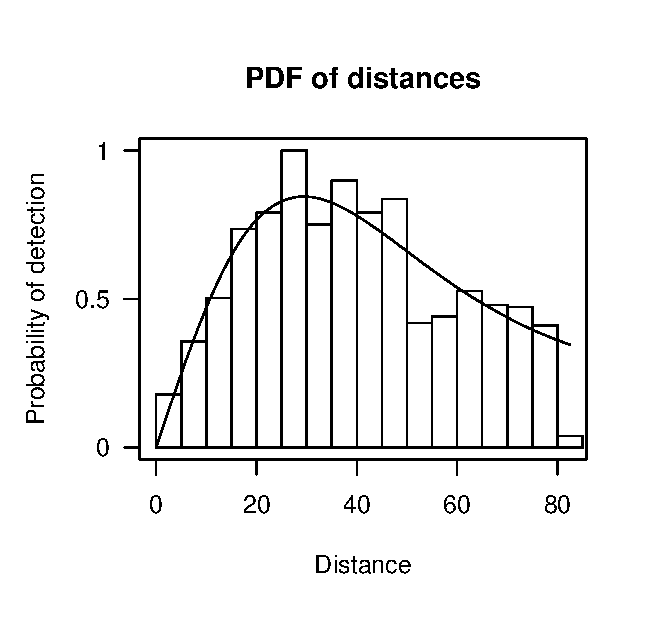
\includegraphics[width=0.4\textwidth]{analyses/amakihi-om-pdf.eps}
\caption{Plots of the (AIC) best mixture model for the amakihi data: a 2-point mixture with observer and minutes after sunrise as covariates. Top row: detection function averaged over covariates (dashed lines are each mixture component averaged over covariates), marginal detection function showing the levels of observer (averaged over the values of minutes after sunrise) and marginal detection function for the quantiles minutes after sunrise (averaged over the levels of observer). Bottom row: pdf of distances averaged over the covariate values.}
\label{amakihi}
\end{figure}

Best mixture model according to AIC was a two point mixture with observer and minutes after sunrise as covariates (shown in Figure \ref{amakihi}), closely followed by the model with only observer as a covariate (see Table \ref{big-results-table}). In this case a hazard-rate with observer and minutes after sunrise as covariates beat the mixtures in AIC terms. This is not too surprising given that the mixtures use one more parameter than a hazard-rate in this situation. It is encouraging that there is such a small difference in AIC, and that covariate mixture models were selected despite the large number of parameters that such models entail.


\begin{table}
\caption{Results for the three data sets with covariates. Bold indicates lowest AIC for each set. In each set the final model is the lowest AIC model reported in the original analysis (using \texttt{mrds}). Kolmogorov-Smirnov test $p$-values (KS $p$) are also given as in Section 11.11 of Buckland \textit{et al.} (2004). Results are from ($i$) the wood ant data from Borkin \textit{et al.} (2012) with truncation at 25m; ($ii$) the long-finned pilot whales Pike et al. (2003) with truncation at 3000m, (cont.) denotes that the covariate was included in the model as continuous, otherwise covariates entered the model as factors; ($iii$) the amakihi data from Marques et al. (2007) with truncation at 82.5m.}
\centering
\begin{tabular}{c l c c c c}
\hline \hline
Model & Covariates & AIC & $\hat{P_a}$ & $\% CV \hat{P_a}$ & K-S $p$\\
\hline
 & ($i$) \textit{Ants} & & & & \\
Hn 2-pt  &  None  &  754.61  &  0.184  &  15.46  &  0.96 \\
Hn 2-pt  &   \texttt{habitat} &  751.27  &  0.188  &  14.85  &  0.97 \\
Hn 2-pt  &   \texttt{species} &  756.59  &  0.184  &  15.48  &  0.94 \\
Hn 2-pt  &  \texttt{nest.size} &  741.64  &  0.214  &  15.19  &  0.76 \\
Hn 2-pt  &  \texttt{habitat} + \texttt{species} &  753.23  &  0.186  &  14.94  &  0.99 \\
Hn 2-pt  &  \texttt{habitat} + \texttt{nest.size}  &  \textbf{737.27}  &  0.179  &  17.55  &  0.72 \\
Hn 2-pt  & \texttt{nest.size} + \texttt{species}   &  741.92  &  0.21  &  15.84  &  0.77 \\
Hn 2-pt  &  \texttt{nest.size} + \texttt{species} + \texttt{habitat}  &  739.08  &  0.178  &  18.09  &  0.83 \\
% Hr & \texttt{nest.size} + \texttt{habitat} & 745.2 & 0.194 & 10.6 & 0.95\\  % Distance result 
Hr & \texttt{nest.size} + \texttt{habitat} & 743.56 & 0.195  & 21.72 & 0.89\\ % mrds result
 & ($ii$) \textit{Long-finned pilot whales} & & & & \\
Hn 2-pt  &  None  &  1298.42  &  0.295  &  17.17  &  0.95 \\
Hn 2-pt  &  \texttt{BSS}  &  1286.59  &  0.209  &  125794.8  &  0.82 \\
Hn 2-pt  &  \texttt{BSS2}  &  1284.99  &  0.211  &  23.39  &  0.95 \\
Hn 2-pt  &  \texttt{BSS3}  &  1296.27  &  0.27  &  17.46  &  0.99 \\
Hn 2-pt  &  \texttt{BSS}  &  \textbf{1284.56}  &  0.216  &  24.17  &  0.67 \\
% Hn 1-pt + $\cos(2)$& \texttt{BSS} (cont.) & 1296 & 0.37 & 9.56 & 0.319 \\ % Distance result 
Hn 1-pt + $\cos(2)$& \texttt{BSS} (cont.) & 1286.5 & 0.452 & 8.69 & 0.48\\ % mrds
 & ($iii$) \textit{Amakihi} & & & & \\
Hn 2-pt  &  None  &  10805.48  &  0.283  &  6.21  &  0.12 \\
Hn 2-pt  & \texttt{obs} &  10778.69  &  0.279  &  5.86  &  0.04 \\
Hn 2-pt  &  \texttt{has}  &  10807.19  &  0.282  &  6.95  &  0.33 \\
Hn 2-pt  &  \texttt{mas}  &  10805.11  &  0.284  &  6.52  &  0.31 \\
Hn 2-pt  &  \texttt{obs} +\texttt{has}  &  10782.53  &  0.283  &  6.21  &  0.23 \\
Hn 2-pt  &  \texttt{obs} +\texttt{mas}  &  \textbf{10778.07}  &  0.279  &  6.1  &  0.14 \\
Hn 2-pt  &  \texttt{mas} +\texttt{has}  &  10809.17  &  0.282  &  6.97  &  0.43 \\
Hn 2-pt  &  \texttt{mas} +\texttt{has}+\texttt{obs}  &  10784.5  &  0.282  &  6.33  &  0.35 \\
% Hr & \texttt{obs} + \texttt{mas} & \textbf{10777.72} & 0.3 & 2.65 & 0.036 \\ % Distance result 
Hr & \texttt{obs} + \texttt{mas} & \textbf{10777.38} &  0.319 & 5.11 & 0.076\\ % mrds
\hline
\hline
\end{tabular}
\label{big-results-table}
\end{table}

\section{Discussion}
\label{s:discuss}

[[\textbf{LEN}: I've put some stuff here but it's a bit rough at the moment. ]]

[[Something here about how you can work out how many there are in each class? See Takis e-mail...]]


We have investigated and demonstrated the utility of detection functions constructed from mixtures of half-normals in both line and point transect distance sampling. We also show that covariates can be included in such models easily. These mixture detection functions can be simply ``dropped in'' to the existing theory. This means mark-recapture distance sampling methods (Laake et al., 2011), spatial models for distance sampling data (Hedley, Buckland and Borchers, 2004), methods for incomplete detection at zero distance (Laake and Borchers, 2004) and other advanced distance sampling methods can exploit this formulation.

We have shown that the method performs well on both simulated and case studies where traditional methods produce unrealistic results. In many cases the proposed model outperformed (M)CDS models in AIC terms, which is surprising given that the mixture models in question often had more parameters. 

Simulations show that small sample sizes do not support the use of mixture models with high number of components, even when the data were generated from such a model. We avoid poorly fitting models of this sort by using AIC forward selection for the number of mixtures, ensuring model parsimony.

In simulation we observed that 3-point mixture did not act as good surrogates for missing covariate structure in the model; 2-point mixtures were generally chosen by AIC as good models. We also note that the construction of a true 3-point mixture is quite tricky. In the examples in Section \ref{s:data}, 2-point mixtures consistently provided the best fit, even in the case of the amakihi data which had many observations ($n=1243$). Only examination of further data will show whether 3-point and higher mixtures can be supported, however we note that when the K$+$A series formulation is used, detection functions with 5 or more parameters are rarely selected by AIC (a 3-point mixture with no covariates requires 5 parameters).

All the models discussed in this article are available as an \textsf{R} package, \texttt{mmds} which is available from \url{http://www.github.com/dill/mmds/}. Mixture model detection functions will be available in the next version of the Distance software.

Further work will include extending these models further to include continuous mixtures. In that case the detection function can be modelled as:
\begin{equation*}
g(x) = \int_\mathbf{R} \varphi(\kappa) g_\kappa(x,\mathbf{Z}; \theta, \kappa) \text{d}\kappa
\end{equation*}
where $\varphi(\kappa)$ is some function which controls the mixing of $g_\kappa$. Such an approach may present significant computation issues, however the benefits of a significantly more flexible detection function may be considerable. Provided that an appropriate function can be chosen for $\varphi$, more flexible models could be used whilst keeping the number of parameters low. In addition, a combination of both finite and continuous mixtures could be used, echoing the work of Morgan and Ridout (2008) in capture-recapture.

[[TKTKTK maybe need to round things up here...]]

%  The \backmatter command formats the subsequent headings so that they
%  are in the journal style.  Please keep this command in your document
%  in this position, right after the final section of the main part of 
%  the paper and right before the Acknowledgements, Supplementary Materials,
%  and References sections. 

\backmatter

%  This section is optional.  Here is where you will want to cite
%  grants, people who helped with the paper, etc.  But keep it short!

\section*{Supplementary material}

Web Appendices referenced in Section \ref{s:likelihood}, \ref{s:popsize} and \ref{s:sims} [[TKTKTK add variance stuff if necessary]] are available with this paper at the Biometrics website on Wiley Online Library.

\section*{Acknowledgements}

David would like to acknowledge the financial support of EPSRC and Simon N. Wood for useful discussions.

Both authors would like to thank David Borchers, who suggested the parametrisation for the mixture proportions as well as Rob Williams, Dan Pike , the amakihi people and the ant people for the data. [[\textbf{LEN}: can you put in the right people to thank here?]]


%  Here, we create the bibliographic entries manually, following the
%  journal style.  If you use this method or use natbib, PLEASE PAY
%  CAREFUL ATTENTION TO THE BIBLIOGRAPHIC STYLE IN A RECENT ISSUE OF
%  THE JOURNAL AND FOLLOW IT!  Failure to follow stylistic conventions
%  just lengthens the time spend copyediting your paper and hence its
%  position in the publication queue should it be accepted.

%  We greatly prefer that you incorporate the references for your
%  article into the body of the article as we have done here 
%  (you can use natbib or not as you choose) than use BiBTeX,
%  so that your article is self-contained in one file.
%  If you do use BiBTeX, please use the .bst file that comes with 
%  the distribution.

\begin{thebibliography}{}

\bibitem{ } Beavers, S. C., and Ramsey, F. L. (1998). Detectability analysis in transect surveys. \textit{Journal of Wildlife Management} \textbf{62}(3), pp. 948--957.

\bibitem{ } Becker, E. F. and Quang, P. X. (2009). A gamma-shaped detection function for line-transect surveys with mark-recapture and covariate data. \textit{Journal of Agricultural, Biological, and Environmental Statistics} \textbf{14}(2), 207--223.

\bibitem{ } Borkin, K.M., Summers, R.W. and Thomas, L. (2012). Distribution, density and stand-type preferences of wood ant Formica spp. nest mounts in a Scots pinewood. \textit{European Journal of Entomology} \textbf{109}: 47--53.

\bibitem{ } Buckland, S.T. (1992). Fitting density functions using polynomials. \textit{Applied Statistics} \textbf{41}, 63--76. 

\bibitem{ }  Buckland, S. T., Anderson, D. R., Burnham, K. P., Laake, J. L., Borchers, D. L., and Thomas, L.  (2001). \textit{Distance Sampling}. Oxford University Press. Oxford, UK.

\bibitem{ }  Buckland, S. T., Anderson, D. R., Burnham, K. P., Laake, J. L., Borchers, D. L., and Thomas, L.  (2004). \textit{Advanced Distance Sampling}. Oxford University Press. Oxford, UK.

\bibitem{ } Dempster, A.P., Laird,  N. M. and Rubin, D. B. (1977). Maximum Likelihood from Incomplete Data via the EM Algorithm. \textit{Journal of the Royal Statistical Society: Series B (Methodological)} \textbf{39}(1), 1--38.

\bibitem{ } Dorazio, R. M. and Royle, J. A. (2003) Mixture Models for Estimating the Size of a Closed Population When Capture Rates Vary among Individuals. \textit{Biometrics} \textbf{59}(2), 351--364 

\bibitem{ }  Gelman, A., Carlin, J. B., Stern, H. S., and Rubin, D. B. (2004). \textit{Bayesian Data Analysis}. CRC Press. Boca Ranton, Florida, US.

\bibitem{ } Hedley, S. L., Buckland, S. T. and Borchers, D. L. (2004). Spatial distance sampling models. In \textit{Advanced Distance Sampling}, pp. 48--70. S. T. Buckland, D. R. Anderson, K. P. Burnham, J. L. Laake, D. L. Borchers and L. Thomas (eds). Oxford University Press, Oxford.

\bibitem{ } Laake, J. L. and Borchers, D. L. (2004). Methods for incomplete detection at distance zero. In \textit{Advanced Distance Sampling}, pp. 108--189. S. T. Buckland, D. R. Anderson, K. P. Burnham, J. L. Laake, D. L. Borchers and L. Thomas (eds). Oxford University Press, Oxford.

\bibitem{ } Laake, J. L., Collier, B. A., Morrison, M. L. and Wilkins, R. N. (2011). Point-Based Mark-Recapture Distance Sampling. \textit{Journal of Agricultural, Biological, and Environmental Statistics}, \textbf{16}(3), 389--408.

\bibitem{ } Mack, Y. P. and Quang, P. (1998). Kernel methods in line and point transect sampling. \textit{Biometrics} \textbf{54}(2), 606--619. 

\bibitem{ } Marques, F. F. C. and Buckland, S. T. (2004). Covariate models for the detection function. In \textit{Advanced Distance Sampling}, pp. 31--47. S. T. Buckland, D. R. Anderson, K. P. Burnham, J. L. Laake, D. L. Borchers and L. Thomas (eds). Oxford University Press, Oxford.

\bibitem{ } Marques, T. A., Thomas, L., Fancy, S. G., Buckland, S. T. (2007). Improving estimates of bird density using multiple-covariate distance sampling. \textit{The Auk} \textbf{124}(9), 1229--1243.

\bibitem{ } Morgan, B. J. T. and Ridout, M. (2008). A new mixture model for capture heterogeneity. \textit{Journal of the Royal Statistical Society: Series C} \textbf{57}(4), 433--446. 

\bibitem{ } Pike, D. G., Gunnlaugsson, T., V\'{i}kingsson, G .A., Desportes, G. and Mikkelson, B.  (2003) An estimate of the abundance of long-finned pilot whales (\textit{globicephala melas}) from the NASS-2001 shipboard survey. Paper SC/11/AE/10 presented to the North Atlantic Marine Mammal Commission (NAMMCO) Scientific Committee Working Group on Abundance Estimates.

\bibitem{ } Pledger, S. (2000). Unified maximum likelihood estimates for closed capture-recapture models using mixtures. \textit{Biometrics} \textbf{56}(2), 434--442. 

\bibitem{ } Pledger, S. (2005). The performance of mixture models in heterogeneous closed population capture-recapture. \textit{Biometrics} \textbf{61}(3), 868--873.

\bibitem{ } Thomas, L., Buckland, S. T., Rexstad, E. A., Laake, J. L., Strindberg, S., Hedley, S. L., Bishop, J. R. B., Marques, T. A. and Burnham, K. P. (2010). Distance software: design and analysis of distance sampling surveys for estimating population size. \textit{Journal of Applied Ecology} \textit{47}, 5--14.

\bibitem{ } Thompson, S. K. (2002). \textit{Sampling}. Wiley, New York, US.

\bibitem{ } Williams, R. and Thomas, L. (2007). Distribution and abundance of marine mammals in the coastal waters of British Columbia, Canada. \textit{Journal of Cetacean Research and Management} \textbf{9}(1), pp. 15--38.

\end{thebibliography}

\label{lastpage}

\end{document}

